\documentclass[varwidth=6.2in,border=3pt]{standalone}
\usepackage{tikz}
\usetikzlibrary{arrows.meta,decorations.pathreplacing,positioning,calc,fit}
\usepackage{amsmath}
\usepackage{algpseudocode}
\usepackage{newtxtext,newtxmath}
\newcommand{\code}[1]{\texttt{#1}}
\newcommand{\truesum}{\code{truesum}}
\begin{document}
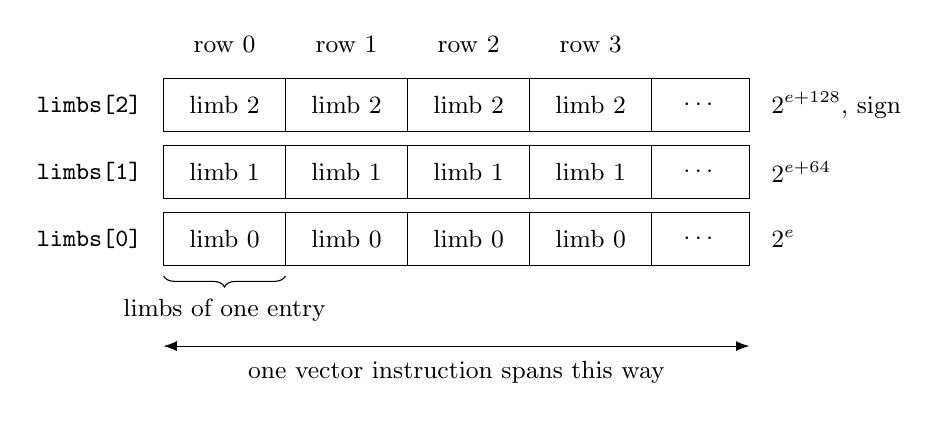
\begin{tikzpicture}[x=1.55cm,y=0.85cm,font=\small]
  \foreach \k/\lab/\sig in {2/limbs[2]/{$2^{e+128}$, sign},1/limbs[1]/{$2^{e+64}$},0/limbs[0]/{$2^{e}$}} {
    \node[anchor=east] at (0,\k) {\code{\lab}};
    \foreach \i in {0,1,2,3} {
      \draw (\i+0.1,\k-0.4) rectangle (\i+1.1,\k+0.4);
      \node at (\i+0.6,\k) {limb \k};
    }
    \draw (4.1,\k-0.4) rectangle (4.9,\k+0.4); \node at (4.5,\k) {$\cdots$};
    \node[anchor=west] at (5.0,\k) {\sig};
  }
  \foreach \i in {0,1,2,3} { \node at (\i+0.6,2.9) {row \i}; }
  \draw[decorate,decoration={brace,mirror,amplitude=4pt}] (0.1,-0.55) -- (1.1,-0.55)
    node[midway,below=5pt] {limbs of one entry};
  \draw[Latex-Latex] (0.1,-1.6) -- (4.9,-1.6) node[midway,below=2pt] {one vector instruction spans this way};
\end{tikzpicture}
\end{document}
